%TODO mettre les nuémros des questions
%TODO : nbepisodes 200 + updatetargetnetwork100

\documentclass[10pt,a4paper]{article}
\usepackage[utf8]{inputenc}
\usepackage[french]{babel}
\usepackage[T1]{fontenc}
\usepackage{amsmath}
\usepackage{amsfonts}
\usepackage{amssymb}
\usepackage{graphicx}
\usepackage{caption}
\usepackage{subcaption}
\usepackage[colorlinks = true, linkcolor = blue, urlcolor  = blue, citecolor = blue, anchorcolor = blue]{hyperref}
\title{Apprentissage profond par renforcement \\ Compte-rendu de TP}
\author{Nelly Barret et Juliette Reisser}

% coding
\usepackage{listings}
\usepackage{xcolor}
\definecolor{codegreen}{rgb}{0,0.6,0}
\definecolor{codegray}{rgb}{0.5,0.5,0.5}
\definecolor{codepurple}{rgb}{0.58,0,0.82}
\definecolor{backcolour}{rgb}{0.95,0.95,0.92}
\lstdefinestyle{mystyle}{
    backgroundcolor=\color{backcolour},   
    commentstyle=\color{codegreen},
    keywordstyle=\color{magenta},
    numberstyle=\tiny\color{codegray},
    stringstyle=\color{codepurple},
    basicstyle=\ttfamily\footnotesize,
    breakatwhitespace=false,         
    breaklines=true,                 
    captionpos=b,                    
    keepspaces=true,                 
    numbers=left,                    
    numbersep=5pt,                  
    showspaces=false,                
    showstringspaces=false,
    showtabs=false,                  
    tabsize=2
}
\lstset{style=mystyle}

% subsubsubsection
\usepackage{titlesec}
\setcounter{secnumdepth}{4}
\titleformat{\paragraph}
{\normalfont\normalsize\bfseries}{\theparagraph}{1em}{}
\titlespacing*{\paragraph}
{0pt}{3.25ex plus 1ex minus .2ex}{1.5ex plus .2ex}


\begin{document}
\maketitle

\tableofcontents

\section{Préliminaires} \label{prelim}
Notre TP se trouve à l'adresse suivante : \href{https://github.com/NellyBarret/IA5-TP-APR}{https://github.com/NellyBarret/IA5-TP-APR}. Pour des raisons de clarté et de concision, la documentation\footnote{Les fichiers Python contiennent la documentation complète.} ainsi que les commentaires ont été retirés du code présent dans ce rapport. Pour les mêmes raisons, certaines parties de code ont étés remplacés par des commentaires (repérables par un \lstinline{##}). \\

Nous avons principalement utilisé les libraires suivantes :
\begin{itemize}
	\item \href{https://gym.openai.com/}{Gym} pour les environnements d'apprentissage
	\item \href{https://keras.io/}{Keras} (de Tensorflow) pour les modèles de réseaux neuronaux
	\item \href{https://numpy.org/}{Numpy} pour les calculs
	\item \href{https://matplotlib.org/index.html}{Matplotlib} pour les tracés de courbe
\end{itemize}
~\\

La suite de cette section décrit les préliminaires du fonctionnement des agents implémentés. Elle se trouve en annexe (section \ref{annexes}) si besoin.

%%%%%%%%%%%%%%%%%%%%%%%%%%%%%%%%%%%%%%%%%%%%%%%%%%%%%%%%%%%%

\section{Compilation et lancement}

Chaque agent est implémenté dans un fichier qui lui est propre. Ainsi il suffit de lancer l'exécution du fichier voulu dans un IDE (e.g. Pycharm). La fonction \lstinline{main} de chaque fichier permet de créer l'environnement et l'agent ainsi que de faire apprendre l'agent sur l'environnement.

%%%%%%%%%%%%%%%%%%%%%%%%%%%%%%%%%%%%%%%%%%%%%%%%%%%%%%%%%%%%

\section{Agent aléatoire sur Cartpole}

Fichier correspondant : \href{https://github.com/NellyBarret/IA5-TP-APR/blob/master/randomCartPole.py}{randomCartpole.py}

\subsection{Définitions et fonctionnalités}
\subsubsection{Définition de l'environnement}
Dans l'environnement CartPole (variable \lstinline{env}), nous avons un bâton posé en équilibre sur un élément que l'on peut faire bouger à gauche ou à droite pour rééquilibrer le bâton. L'objectif principal pour l'agent est de maintenir le bâton assez vertical pour que celui-ci ne tombe pas et/ou ne sorte pas de l'environnement.

Nous allons maintenant spécifier les variables que nous avons défini en section \ref{prelim}.
\begin{itemize}
	\item L'espace des actions est de taille 2 car l'agent peut faire bouger l'élément à gauche (action 0) ou à droite (action 1)
	\item L'espace des états est de taille 4 car il est défini comme suit : [position de l'élément, vitesse de l'élément, angle du bâton, taux de rotation du bâton]
	\item La méthode \lstinline{act()} implémente une politique aléatoire (c.f. section \ref{defAgentRand})
\end{itemize}

\subsubsection{Définition de l'agent} \label{defAgentRand}
L'agent aléatoire suit une politique aléatoire pour choisir l'action qu'il va exécuter dans l'environnement. Il les choisit parmi ses actions possibles (disponibles dans \lstinline{env.action_space}). Il n'a pas de mémoire de ses précédentes expériences, ne prend pas en compte les gains futurs, ... . En somme, il exécute simplement des actions choisies aléatoirement.

\begin{lstlisting}[language=Python, caption=Programme principal de l'agent aléatoire]
env = gym.make("CartPole-v1")
agent = RandomAgent(env.action_space)
nb_episodes = 1000 # (1)
liste_rewards = [] # (2)
for i in range(nb_episodes): 
    total_reward = 0
    env.reset()
    while True: # (3)
        action = agent.act()
        _, reward, done, _ = env.step(action)
        total_reward += reward
        if done:
            break
        liste_rewards.append(total_reward) # (2)
evolution_rewards(liste_rewards)  # (2)
print("Meilleure recompense obtenue", max(liste_rewards), "lors de l'episode", liste_rewards.index(max(liste_rewards))) # (2)
env.close()

\end{lstlisting}

Le code ci-dessus montre l'instanciation du pseudo-code de l'entraînement d'un agent (en section \ref{prelim}).

\begin{lstlisting}[language=Python]
# (1)
\end{lstlisting}
Nous devons choisir le nombre d'épisode sur lequel l'agent va s'entraîner. Comme l'agent a une politique aléatoire, le nombre d'épisode n'est pas un facteur influant les performances de l'agent puisque celui-ci exécute toujours des actions choisies aléatoirement. Nous prendrons comme paramètre 1000, ce qui permet de vérifier que l'agent interagisse correctement avec l'environnement sans pour autant que cela n'augmente de manière significative le temps d'exécution.

\begin{lstlisting}[language=Python]
# (2)
\end{lstlisting}
Cette partie traite de l'évolution de la somme des récompenses perçues par l'agent. Pour chaque épisode nous ajoutons la récompense obtenue pour l'action choisie ce qui permet d'avoir une récompense \og globale \fg{}  par épisode. La fonction \lstinline{evolution_rewards} permet de tracer la courbe correspondant à ces récompenses par épisode. Nous avons aussi récupéré la meilleure somme de récompense obtenue ainsi que le numéro de l'épisode où elle a été obtenue (ligne 16).

\begin{lstlisting}[language=Python]
# (3)
\end{lstlisting}
Dans cette partie là du code, nous rentrons dans un épisode. Dans cet épisode, l'agent devra choisir une action puis l'exécuter dans l'environnement. La première étape est faite par la méthode \lstinline{act()}. Comme l'agent suit une politique aléatoire celle-ci retourne simplement une action parmi celles de l'espace d'actions de l'agent. Cela se traduit par le code ci-dessous :

\begin{lstlisting}[language=Python, caption=Implémentation de l'agent aléatoire]
class RandomAgent:
    def __init__(self, action_space):
        ## assignation des parametres a leur variable eponyme

    def act(self):
        return self.action_space.sample()
\end{lstlisting}
Après avoir choisi une action, l'agent l'exécute dans l'environnement via la fonction \lstinline{step}, ce qui lui permettra d'obtenir une récompense (ajoutée à la somme des récompenses de l'épisode en cours) et le booléen \lstinline{done}. Si ce booléen s'évalue à vrai, l'épisode se termine et le suivant commence. Sinon l'épisode continue et l'agent choisit une nouvelle action.

\subsection{Analyse de performances}


Pour évaluer notre agent aléatoire, nous avons réalisé un graphique traçant la somme des récompenses obtenues pour chaque épisode.

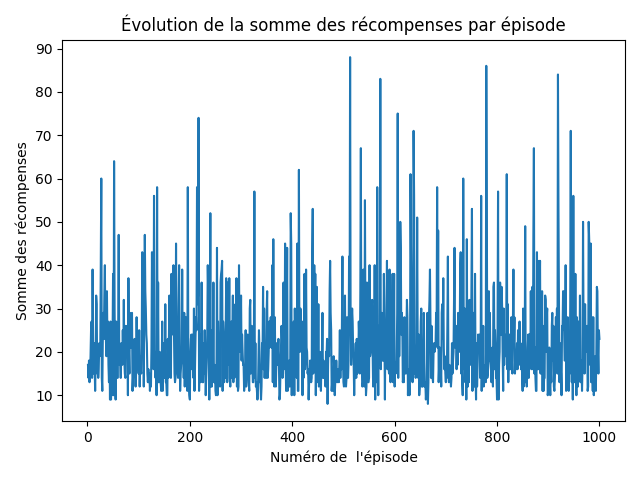
\includegraphics[scale=0.5]{evolution_recompenses_random.png} 

La courbe bleue représente la somme des récompenses obtenue pour chaque épisode. La courbe orange représente la moyenne des récompenses pour les \lstinline{nb_episodes} épisodes. Nous pouvons observer qu'il n'y a pas de tendance particulière. Cela semble cohérent avec le fait que l'agent n'a aucun moyen d'apprendre de ses erreurs (pas de mémoire ni de rétro-propagation) et qu'il ne choisisse pas les meilleures actions (politique aléatoire). 

\subsection{Experience replay}

Fichier correspondant : \href{https://github.com/NellyBarret/IA5-TP-APR/blob/master/ExperienceReplayAgent.py}{ExperienceReplayAgent.py}

Cet agent choisit aléatoirement ses actions et implémente une mémoire ce qui lui permettra par la suite d'apprendre par rapport à ses expériences passées.

\subsubsection{Définition de la mémoire}

\begin{lstlisting}[language=Python, caption=Implémentation de la mémoire d'un agent]
class Memory:
    def __init__(self, max_size, batch_size):
        ## assignation des parametres a leur variable eponyme
        self.memory = [[] for _ in range(self.max_size)]
        self.position = 0

    def add(self, state, action, reward, next_state, done):
        self.memory[self.position] = [state, action, reward, next_state, done]
        self.position = (self.position + 1) % self.max_size

    def sample(self):
        if self.__len__() < self.batch_size:
            return None
        else:
            batch = random.sample(self.memory, self.batch_size)
            return batch

    def __len__(self):
        return sum(len(item) > 0 for item in self.memory)
\end{lstlisting}

Cette classe définit la mémoire de l'agent. Elle stocke sous forme de liste les expériences que l'agent a avec l'environnement. Chaque expérience est une liste de 5 éléments : l'état courant de l'agent (variable \lstinline{state}), l'action choisie par l'agent (variable \lstinline{action}), la récompense obtenue pour cette action (variable \lstinline{reward}), l'état dans lequel va arriver l'agent après exécution de l'action (variable \lstinline{next_state}) et la variable \lstinline{done} qui indique si l'agent a terminé l'épisode ou non. Une expérience se formalise ainsi :

$$
expe_i = [state_i, action_i, reward_i, nextstate_i, done_i]
$$

Cette mémoire a un nombre maximal d'éléments (variable \lstinline{max_size}), donc quand un nouvel élément est inséré et qu'il n'y a plus de place, ce nouvel élément remplace le plus ancien. Elle se formalise comme suit : 

$$
memory = \bigcup\limits_{i=1}^{max\_size} expe_{i} = 
\begin{bmatrix}
[state_1, action_1, reward_1, nextstate_1, done_1] \\
... \\
[state_n, action_n, reward_n, nextstate_n, done_n]
\end{bmatrix}
$$

De plus, nous avons deux fonctions pour interagir avec la mémoire :
\begin{itemize}
	\item \textit{L'ajout d'une nouvelle expérience} via la fonction \lstinline{add(...)} : cela ajoute à la mémoire de l'agent ce qu'il vient d'expérimenter dans l'environnement. Ce processus lui permettra par la suite d'apprendre de ses expériences passées.
	\item \textit{La création d'un batch} via la fonction \lstinline{sample()}: cette fonctionnalité crée un batch d'expériences en choisissant des éléments de manière aléatoire dans la mémoire.
\end{itemize}

Enfin, deux conditions sont à respecter :
\begin{enumerate}
	\item Le dépassement de la taille maximale doit être prévu. Il est prévu par le modulo utilisé pour la position de la nouvelle expérience à insérer. En effet, quand la mémoire arrive à sa capacité maximale, la position revient à 0, ce qui permet de remplacer les plus anciennes expériences par les nouvelles.
	\item La mémoire est indépendante de l’environnement, et donc de l’espace d’action et d’état. Cette condition est respectée par l'insertion au fur et à mesure dans la mémoire et le fait de n'avoir qu'une taille maximale comme condition.
\end{enumerate}

\subsubsection{Définition de l'agent}

\begin{lstlisting}[language=Python, caption=Implémentation de l'agent utilisant son expérience]
class ExperienceReplayAgent:
    def __init__(self, action_space, batch_size):
        ## assignation des parametres a leur variable eponyme
        self.memory = Memory(100, self.batch_size)
        
    def act(self):
        return self.action_space.sample()

    def remember(self, state, action, reward, next_state, done):
        self.memory.add(state, action, reward, next_state, done)

    def creer_batch(self):
        return self.memory.sample()
\end{lstlisting}

Comme vu précédemment, cet agent redéfinit la méthode \lstinline{act()} et se base toujours sur une politique aléatoire. Cet agent a une fonctionnalité supplémentaire, celle de se souvenir d'une expérience grâce à la fonction \lstinline{remember(...)} qui permet d'ajouter une expérience à sa mémoire, comme définit ci-dessus.

\begin{lstlisting}[language=Python, caption=Programme principal de l'agent utilisant l'expérience replay]
## creation de l'environnement et de l'agent
nb_episodes = 100
for i in range(nb_episodes):
    env.reset()
    while True:
        action = agent.act()
        next_state, reward, done, _ = env.step(action)
        agent.remember(state, action, reward, next_state, done)
        if done:
            break
    batch = agent.creer_batch()
    env.close()
\end{lstlisting}

Enfin, nous devons modifier quelque peu le programme principal afin que l'agent enregistre les nouvelles expériences qu'il a avec l'environnement. Le squelette (créations de l'environnement et de l'agent, boucle sur le nombre d'épisodes, boucle pour chaque épisode) ne change pas. En revanche l'agent ajoute chacune de ses expériences dans sa mémoire grâce à la fonction \lstinline{remember(...)}. Après avoir réalisé tous les épisodes, l'agent peut créer le batch sur sa mémoire. La création du batch est simplement un tirage aléatoire de n expériences où n est la taille du batch. Par exemple, ici nous créons un batch de 20 expériences (défini lors de la création de l'agent).


%%%%%%%%%%%%%%%%%%%%%%%%%%%%%%%%%%%%%%%%%%%%%%%%%%%%%%%%%%%%

\section{Deep Q-learning sur CartPole}

Dans la section précédente nous avons défini le problème du CartPole ainsi qu'un agent basique qui choisit aléatoirement ses actions. Nous lui avons ensuite ajouté  une mémoire en vu qu'il puisse apprendre de ses expériences passées. Nous allons maintenant lui faire apprendre de ses expériences en lui implémentant un algorithme d'apprentissage profond de type Q-learning.

\subsection{Construction du modèle neuronal}

\subsubsection{Définition du modèle}
Pour le code, voir la fonction \lstinline{build_model()} en \ref{modeleneuronal}.

Dans un premier temps, nous avons construit le modèle neuronal de notre agent. La taille de l'entrée est égale à la taille d'un état (en l'occurence 4 pour CartPole) et la taille de sortie est égale aux nombre d'actions (2 pour CartPole). Nous avons une seule couche cachée de taille 24 et qui a pour fonction d'activation \lstinline{ReLu}, i.e. que les neurones s'activent sur les entrées positives car la fonction ReLu peut se formaliser ainsi :

$$ReLu(x) = \max \{0, x\} \text{ où } x \text{ est une entrée}$$

Nous avons aussi une fonction d'erreur, ici nous avons choisi \lstinline{mse}, i.e. mean squared error. Cette fonction d'erreur calcule la moyenne des différences au carré entre les valeurs prédites et les valeurs cibles. Cette fonction est la métrique par défaut lorsqu'il s'agit de réseaux neuronaux de ce type, c'est pourquoi nous avons choisi celle-ci.

\subsubsection{Paramétrage du modèle}

Afin de trouver les meilleurs paramètres pour notre modèle neuronal, nous avons effectué plusieurs tests. Ci-dessous un tableau récapitulant les paramètres testés ainsi que leurs résultats :
\begin{table}[!h]
\begin{tabular}{|p{0.7cm}|p{2.3cm}|p{2.3cm}|p{2.3cm}|p{2.3cm}|}
\hline
Expé & Taille de la couche cachée & Fonction d'activation & Utilisation du target network & Meilleure récompense obtenue sur un épisode \\ \hline
1    & 24                         & ReLu                  & Oui                           & 72                                          \\ \hline
2    & 30                         & ReLu                  & Oui                           & 99                                          \\ \hline
3    & 1024                       & ReLu                  & Oui                           & 119                                         \\ \hline
4    & 24                         & TanH                  & Oui                           & 50                                          \\ \hline
5    & 24                         & ReLu                  & Non                           & 87                                          \\ \hline
\end{tabular}
\end{table}

Voir la section \ref{graphDQN} pour les graphiques correspondants.

\subsection{Construction de l'agent}

\subsubsection{Définition de l'agent} \label{modeleneuronal}

La construction de cet agent se base donc sur un modèle de réseau neuronal et une mémoire. Les paramètres utilisés sont détaillés dans la section suivante en \ref{paramDQN}

\begin{lstlisting}[language=Python, caption=Programme principal de l'agent utilisant l'expérience replay]
class DQNAgent:
    def __init__(self, params):
        ## assignation des parametres a leur variable eponyme

        self.model = self.build_model()
        self.target_model = self.build_model()

    def build_model(self):
        model = Sequential()
        model.add(Dense(24, input_dim=self.state_size, activation='relu'))
        model.add(Dense(24, activation='relu'))
        model.add(Dense(self.action_size, activation='linear'))
        model.compile(loss='mse', optimizer=Adam(lr=self.learning_rate))
        return model

	# (1)
    def act(self, state, policy="greedy"):
        if policy == "greedy":
            ## politique e-greedy
        elif policy == "boltzmann":
            ## politique Boltzmann
        else:
            return env.action_space.sample()

    def remember(self, state, action, reward, next_state, done):
        self.memory.add(state, action, reward, next_state, done)

	# (2)
    def experience_replay(self):
        ## experience replay avec calcul des q-valeurs
    
    # (3)
    def update_target_network(self):
        self.target_model.set_weights(self.model.get_weights())
\end{lstlisting}

\begin{lstlisting}[language=Python]
# (1)
\end{lstlisting}

Voir section \ref{politiquesDQN}

\begin{lstlisting}[language=Python]
# (2)
\end{lstlisting}

Voir section \ref{qvalDQN}

\begin{lstlisting}[language=Python]
# (3)
\end{lstlisting}

Voir section \ref{targetmodelDQN}

~\\

Le programme principal de l'agent DQN reprend le pseudo-code donné en section \ref{prelim}. Pour chaque épisode, l'agent choisit une action, la réalise dans l'environnement, ajoute cette nouvelle expérience à sa mémoire et comptabilise ses récompenses.
\begin{lstlisting}[language=Python, caption=Programme principal de l'agent DQN]
## creation de l'environnement "CartPole-v1" et de l'agent avec ses parametres
liste_rewards = []
global_counter = 0
    for i in range(nb_episodes):
        state = env.reset()
        steps = 1
        sum_reward = 0
        while True:
            action = agent.act(state, "greedy")
            next_state, reward, done, _ = env.step(action)
            agent.remember(state, action, reward, next_state, done)
            state = next_state
            sum_reward += reward
            agent.experience_replay()
            if done:
                print("Episode", i,"- nombre de pas : ", steps, "- somme recompenses", sum_reward)
                break
            if global_counter % update_target_network == 0:
                agent.update_target_network()
            steps += 1
            global_counter += 1
        liste_rewards.append(sum_reward)
        if save_weights and i % save_step == 0:
            agent.model.save_weights("./cartpole_dqn.h5")
    evolution_rewards(liste_rewards)
    print("Meilleure recompense obtenue", max(liste_rewards), "lors de l'episode", liste_rewards.index(max(liste_rewards)))
\end{lstlisting}

\subsubsection{Paramétrage de l'agent} \label{paramDQN}
Nous avons plusieurs paramètres à prendre en compte et à ajuster à la résolution du problème de CartPole. Ces paramètres sont les suivants : 
\begin{itemize}
	\item La taille de la mémoire (\lstinline{memory_size}) : si la mémoire est trop petite, les batchs construits auront beaucoup de ressemblance (du fait de la petite taille de l'espace de tirage) donc le réseau apprendra peu. Par défaut la taille de la mémoire est fixée à 100000.
    \item La taille du batch (\lstinline{batchsize}) : c'est sur ce batch que le réseau va se mettre à jour et donc apprendre. Si le batch est trop petit, le réseau apprendra peu ; s'il est trop grand, le temps d'apprentissage sera considérable.
    \item Le gamma qui définit l'importance des récompenses à l'infini. Plus ce paramètre est proche de 1, plus l'agent aura tendance à attendre une meilleure récompense dans les états futurs (il privilégie une plus grosse récompense lointaine). Inversement, plus ce paramètre est proche de 0 plus l'agent va privilégier les récompenses proches. Nous l'avons défini à 0.99 afin de prendre en compte les récompenses lointaines.
    \item Le taux d'apprentissage (\lstinline{learning_rate}) : nous l'avons défini à 0.001, valeur communément acquise par la communauté scientifique. Ce taux permet de plus ou moins apprendre l'erreur (entre la prédiction que le réseau a fait et la valeur cible).
    \item Le taux d'exploration (\lstinline{exploration_rate}) est utilisé dans les stratégies $\epsilon$-greedy et Boltzmann. Ce taux permet de choisir si l'agent va faire une action aléatoire ou l'action qu'il prédit comme meilleure. Dans le premier cas, cela permet de diversifier l'apprentissage, i.e. d'explorer de nouveaux états. Dans le second, cela permet d'intensifier l'apprentissage, i.e. de rester dans des états proches pour augmenter la somme des récompenses. Ce taux débute à 1 puis est diminué par le facteur \lstinline{exploration_decay} (0.995) jusqu'à son minimum \lstinline{exploration_min} (0.01). Cela permet notamment de faire baisser le nombre d'explorations au fur et à mesure que l'agent apprend et devient meilleur.
    \item Le nombre d'épisode est maintenant mis à 200 car le problème du CartPole est considéré comme résolu si un score de 195 a été atteint avant 200 épisodes.
    \item Le target network est mis à jour toutes les 100 itérations (au global). Cela permet au réseau de se remettre à jour assez souvent pour apprendre mais de rester dans des temps d'apprentissage raisonnables.
\end{itemize}

\begin{lstlisting}[language=Python, caption=Paramétrage de l'agent DQN]
if __name__ == '__main__':
    ## creation de l'environnement "CartPole-v1"
    
    nb_episodes = 200
    update_target_network = 100
    params = {
        'state_size': env.observation_space.shape[0],
        'action_size': env.action_space.n,
        'memory_size': 100000,
        'batch_size': 64,
        'gamma': 0.99,
        'learning_rate': 0.001,
        'exploration_rate': 1,
        'exploration_decay': 0.995,
        'exploration_min': 0.01
    }
    agent = DQNAgent(params)
\end{lstlisting}

\subsubsection{Politiques} \label{politiquesDQN}

La fonction \lstinline{act(...)} définit maintenant deux politiques : $\epsilon$-greedy et Boltzmann (et aléatoire le cas échéant). La politique est donnée comme paramètre à la fonction \lstinline{act(...)} et peut prendre comme valeurs \lstinline{greedy} ou \lstinline{boltzmann}. Nous allons maintenant détailler chacune de ces deux politiques.

La politique $\epsilon$-greedy permet soit d'explorer les états en renvoyant une action aléatoire soit d'intensifier l'apprentissage en renvoyant la meilleure action prédite par la réseau. En comparaison de la poitique greedy, elle a l'avantage d'explorer les possibilités en choisissant des actions aléatoires.
\begin{lstlisting}[language=Python, caption=Politique e-greedy]
if numpy.random.rand() < self.exploration_rate:
    return random.randrange(self.action_size)
else:
    q_values = self.model.predict(state)
    return numpy.argmax(q_values[0])
\end{lstlisting}    

La politique de Boltzmann permet de choisir une action $a_k$ selon la probabilité définie comme suit :

 $$P(s, a_k) = \frac{e^{\frac{Q(s,a_k)}{\tau}}}{\sum_ie^{\frac{Q(s,a_i))}{\tau}}}$$
 
Plus $\tau$ est grand, plus la politique aura tendance à être aléatoire puisque le quotient $\frac{Q(s,a_k)}{\tau}$ tendra vers 0 donc la quotient donnant la probabilité de Boltzmann donnera des probabilités assez proches. Avec des probabilités proches, cela revient à choisir une action aléatoirement puisqu'aucune ne se distingue des autres. Inversement, plus $\tau$ est petit, plus les écarts entre probabilités seront forts, ce qui permettra de choisir la meilleure action avec une grande probabilité.

\begin{lstlisting}[language=Python,caption=Politique de Boltzmann]          
if numpy.random.rand() <= self.exploration_rate:
    return env.action_space.sample()
else:
    tau = 0.8
    q_values = self.model.predict(state)
    sum_q_values = 0
    boltzmann_probabilities = [0 for _ in range(len(q_values[0]))]
    for i in range(len(q_values[0])):
        sum_q_values += numpy.exp(q_values[0][i] / tau)
    for i in range(len(q_values[0])):
        current_q_value = q_values[0][i]
        boltzmann_probabilities[i] = numpy.exp(current_q_value/tau) / sum_q_values
    return numpy.argmax(boltzmann_probabilities)
\end{lstlisting}

\subsubsection{Calcul des Q-valeurs} \label{qvalDQN}
Le calcul des Q-valeurs se base sur l'équation de Bellman qui se définit ainsi :
$$Q(s,s',a,a') = r(s,a) + \gamma * max_{a'}Qt(s', a')$$ où $Q$ est le réseau de neurones, $Qt$ le target network, $s$ et $s'$ des états, $a$ et $a'$ des actions, $r$ la fonction de récompense. 

L'idée de cette fonction est d'apprendre sur les expériences passées. Dans un premier temps, on construit le batch sur lequel on va apprendre. Ensuite, en le parcourant, on calcule les Q-valeurs de chaque action pour un état donné en appliquant la formule de Bellman. Quand l'épisode se termine, l'équation de Bellman se résume à la récompense puisqu'il n'existe pas de prochain état. La ligne 3 prédit les valeurs des différentes actions avec le modèle courant. Après avoir calculé la Q-valeur de l'action, on met à jour le réseau (ligne 8). Enfin, le réseau réajuste ses poids grâce à la fonction \lstinline{fit}. Après avoir parcouru tout le batch, on met à jour le taux d'exploration (voir section \ref{paramDQN}).

\begin{lstlisting}[language=Python, caption=Expérience repaly de l'agent DQN]
## creation du batch dans la variable batch
for state, action, reward, state_next, done in batch:
	q_values = self.model.predict(state)
	if done:
		q_update = reward
	else:
		q_update = reward + self.gamma * numpy.max(self.target_model.predict(next_state)[0])
	q_values[0][action] = q_update
	self.model.fit(state, q_values, verbose=0)
## mise a jour du taux d'exploration
\end{lstlisting}

\subsubsection{Target model} \label{targetmodelDQN}

Nous avons pu observer que l'agent apprend des comportements intéressants mais qu'il n'était pas très stable. Dans cette optique, nous avons ajouté un second réseau (\lstinline{target_network}) dans le but de stabiliser le réseau. Ce réseau se base sur le même modèle que l'original. La mise à jour est une recopie des poids du réseau de base dans le target network (voir section \ref{paramDQN}).

\section{Breakout Atari}

Dans le problème du Breakout, le but est d'éliminer toutes les briques en les touchant avec une balle. Le balle rebo,ndit sur une plateforme et c'est cette plateforme qu'il faut drigier à droite et à gauche pour faire rebondir la balle et continuer à jouer. Un comportement intéressants serait de casser les briques d'un côté pour faire passer la balle derrière le mur de briques. 

\subsection{Définition de l'environnement}

\subsection{Définition de l'agent}

\subsubsection{Préprocessing des états}

Il est important d'avoir une étape de pré-processing afin de \og simplifier \fg{} les frames, i.e. de les passer en noir et blanc puis de les réduire afin de limiter l'explosion lors de l'apprentissage. Ci-dessous le code correspond à ces deux étapes.

\begin{lstlisting}[language=Python,caption=Préprocessing des états]
def preprocessing(observation):
    observation = cv2.cvtColor(cv2.resize(observation, (84, 110)), cv2.COLOR_BGR2GRAY)
    observation = observation[26:110, :]
    ret, observation = cv2.threshold(observation, 1, 255, cv2.THRESH_BINARY)
    return numpy.reshape(observation, (84, 84, 1))
\end{lstlisting}

\subsubsection{Réseau convolutionnel}

Pour notre agent apprenant à jouer au Breakout, nous avons remplacé le réseau entièrement connecté (avec \lstinline{Dense}) par une réseau convolutionnel. Nous avons choisi d'en mettre 3 car cela semble le meilleur paramètres en terme de performances. Chaque couche s'active avec la fonctin ReLu. Afin d'aplanir la dernière couche nous utilisons la fonction \lstinline{Flatten()}. Enfin, la dernière couche est de la taille du nombre d'actions. Nous utilisons encore la fonction \lstinline{mse} pour l'erreur.

\begin{lstlisting}[language=Python]
input_shape = (84, 84, 1)
self.model = Sequential()
self.model.add(Conv2D(32, 8, strides=(4, 4), padding="valid", activation="relu", input_shape=input_shape, data_format="channels_first"))
self.model.add(Conv2D(64, 4, strides=(2, 2), padding="valid", activation="relu", input_shape=input_shape, data_format="channels_first"))
self.model.add(Conv2D(64, 3, strides=(1, 1), padding="valid", activation="relu", input_shape=input_shape, data_format="channels_first"))
self.model.add(Flatten())
self.model.add(Dense(512, activation="relu"))
self.model.add(Dense((self.action_size,)))
self.model.compile(loss="mse", optimizer=RMSprop(lr=0.00025, rho=0.95, epsilon=0.01), metrics=["accuracy"])
\end{lstlisting}

\section{Annexes} \label{annexes}

\subsection{Préliminaires - suite}


Dans cette section préliminaire, nous allons définir quelques variables communes aux différentes implémentations. Ces variables font partie de la logique même utilisée par Gym.

Nous avons accès à deux variables importantes quant à la définition de l'environnement :
\begin{itemize}
	\item L'\textbf{espace des actions} (\lstinline{env.action_space}) qui définit les actions possibles pour l'agent. Chaque action est un entier, e.g. 0 pour aller à gauche, 1 pour aller à droite.
	\item L'\textbf{espace des observations}, ou \textbf{espace d'états}, (\lstinline{env.observation_space}) qui définit un tableau représentant les métriques importantes de l'environnement, e.g. la position d'un élément, les frames d'un jeu...
\end{itemize}

Nous avons aussi 3 variables importantes quant à l'exécution d'actions sur l'environnement :
\begin{itemize}
	\item \lstinline{next_state} qui définit le \textbf{nouvel état} (après exécution de l'action sur l'environnement)
	\item \lstinline{reward} qui représente la \textbf{récompense} gagnée par l'agent après exécution de l'action sur l'environnement
	\item \lstinline{done} qui est un booléen indiquant si l'épisode courant est fini, e.g. le bâton est tombé
\end{itemize}

Enfin, nous avons deux méthodes importantes quant à la communication environnement/agent :
\begin{itemize}
	\item \lstinline{act()} qui retourne l'\textbf{action} choisie par l'agent. C'est dans cette fonction que nous implémenterons les \textbf{politiques} (de sélection d'action), i.e. aléatoire, $\epsilon$-greedy et Boltzmann. 
	\item \lstinline{step(action)} qui exécute une action sur l'environnement et retourne les 3 variables expliquées ci-dessus. 
\end{itemize}

Maintenant que nous avons défini les variables importantes, nous allons définir le fonctionnement général des agents.

\begin{lstlisting}[language=Python, caption=Pseudo-code du fonctionnement de l'agent dans son environnement]
env = gym.make("nom-environnement")
agent = Agent()

Pour chaque episode dans (0, nb_max_epsiodes), Faire
    Tant que True, Faire:
        action = agent.act()
        next_state, reward, done, info = env.step(action)
        Si done == True, Faire:
            break
\end{lstlisting}

Dans un premier temps il est important de créer l'environnement voulu dans la variable \lstinline{env} et de créer un agent. C'est cet agent que nous allons entraîner dans l'environnement.
Le principe de l'entraînement de l'agent est le suivant : l'agent va interagir avec l'environnement pendant \lstinline{nb_max_epsiodes} épisodes. Un épisode correspond à toutes les actions que l'agent va pouvoir faire jusqu'à ce qu'une condition ne soit plus respectée (e.g. le bâton est tombé). Un épisode est donc une boucle qui se termine grâce à une condition, ici c'est \lstinline{done}. Durant cette boucle, l'agent choisit une nouvelle action à faire grâce à sa fonction \lstinline{act()} puis l'exécute d'ans l'environnement avec la fonction \lstinline{step(action)}. Pour résumer, un épisode est défini par la boucle \lstinline{Tant que} et l'agent s'entraîne pendant \lstinline{nb_max_episodes} épisodes.

\subsection{Tracés du paramétrage du DQN} \label{graphDQN}

La légende est sous la forme :
$$ < \text{taille de la couche cachée, fonction d'activation, utilisation du target network} >$$

\begin{center}
	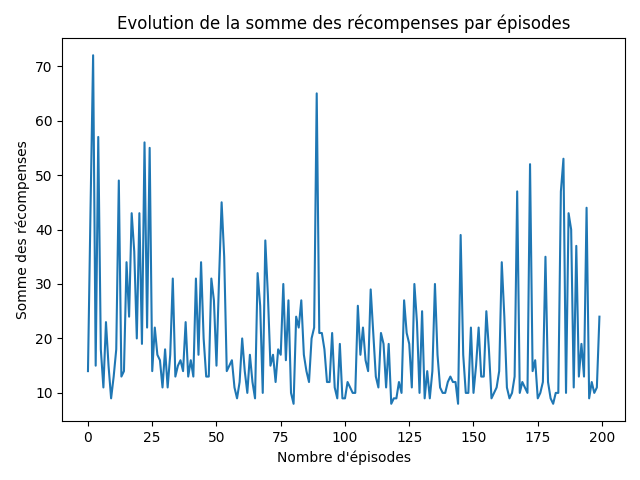
\includegraphics[scale=0.3]{tarnetRelu24.png}
	\captionof{figure}{< 24, ReLu, oui >}
\end{center}

\begin{minipage}{.5\textwidth}
  \centering
  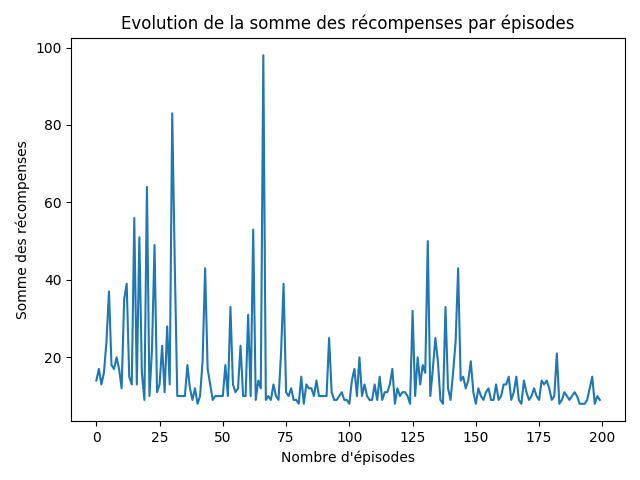
\includegraphics[scale=0.3]{tarnetRelu30.png}
  \captionof{figure}{< 30, ReLu, oui >}
\end{minipage}%
\begin{minipage}{.5\textwidth}
  \centering
  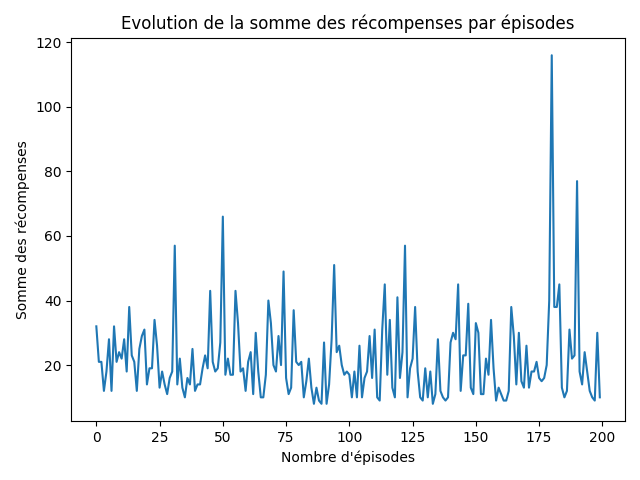
\includegraphics[scale=0.3]{tarnetRelu1024.png}
  \captionof{figure}{< 1024, ReLu, oui >}
\end{minipage}

\begin{minipage}{.5\textwidth}
  \centering
  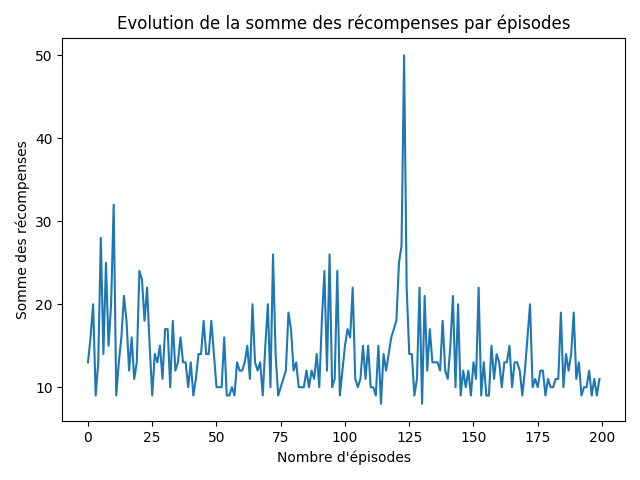
\includegraphics[scale=0.3]{tarnetTanh24.png}
  \captionof{figure}{< 24, Tanh, oui >}
\end{minipage}%
\begin{minipage}{.5\textwidth}
  \centering
  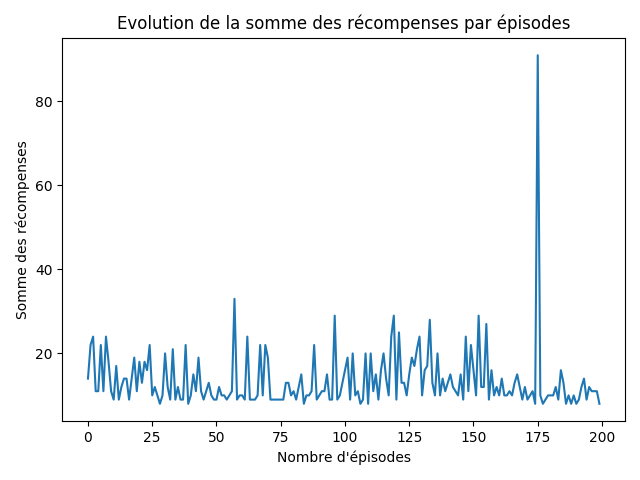
\includegraphics[scale=0.3]{netRelu24.png}
  \captionof{figure}{< 24, ReLu, non >}
\end{minipage}


\end{document}
